\chapter{Results} \label{chapter:interviews}

It should not be surprising that neither data scientists nor software engineers can be replaced by software libraries. However, a non-negligible subset of their processes can be partially or fully automated, especially, when it comes to packaging and deploying AI/ML services. My goal was to design a library with an API that finds the balance between being simple enough to adopt without friction, yet useful/powerful enough to be adopted. Simplicity is subjective and it will be discussed separately in Section \ref{section:interviews}. For now, let us look at the utility of \textit{GreatAI}.

\section{Features} \label{section:features}

For answering \textbf{RQ3} --- \textit{To what extent can \textit{GreatAI} automatically implement AI deployment best practices?} --- a comparison is presented in the following that illustrates which best practices can be implemented/scaffolded/configured with little user input; hence, through a simple and streamlined API. Tables \ref{table:best-practices-1} and \ref{table:best-practices-2} summarise the implemented best practices in the context of methods found by prior surveys of scientific and grey literature \cite{serban2020adoption,serban2021practices,john2020architecting}.

In order to show an accurately nuanced representation, a \textit{Level of support} is determined for each best practice on a scale of \textit{Fully automated}, \textit{Supported}, and \textit{Partially supported}. For instance, \textit{Use static analysis to check code quality} from Table \ref{table:best-practices-1} is \textit{Supported} because the entire public interface of \textit{GreatAI} is correctly typed (including generics and asynchronous coroutines) and compatible with \href{https://mypy.readthedocs.io/en/stable/index.html#}{\texttt{mypy}} and \href{https://marketplace.visualstudio.com/items?itemName=ms-python.vscode-pylance}{\texttt{Pylance}}. This means that when \textit{GreatAI} is used in any Python project, these tools can be applied to statically check the soundness of the project's integration with \textit{GreatAI}. However, if the library's user does not use typehints in their code and it contains a more complex control flow, it can only be partially type-checked. In short, this best practice is supported, and a considerable part of it is already implemented by \textit{GreatAI}, but clients should still keep in mind that they might also need to make effort to fully implement it.

This is not the case for \textit{Log production predictions with the model's version and input data} because by default, it is automatically implemented when calling \texttt{@GreatAI.create}. Users can still specify the exact expected behaviour, e.g.: where to store traces, additional metrics to log, or disabling the logging of sensitive input. Nevertheless, without input from the library's user, the best practice is already reasonably well implemented.

\begin{table}
\centering
\begin{threeparttable}
\caption{A subset of AI lifecycle best practices and the level of support \textit{GreatAI} provides for them. The level of support is one of \textit{Fully automated} (\checkmark\checkmark) which means that no action is required from the user, \textit{Supported} (\checkmark) only automates the reasonably automatable aspects, while \textit{Partially supported} ($\sim$) provides some useful features but the client is expected to build on top of these.}

\label{table:best-practices-1}
{\renewcommand{\arraystretch}{1.2} % for the vertical padding
\begin{tabular}{p{7cm}@{\hskip 0.5cm}l@{\hskip 0cm}c} \hline

\textbf{Best practice}                                                                    & \textbf{Implementation}                        & \textbf{Support}       \\\hline
Use sanity checks for all external data sources\textsuperscript{1}                        & \texttt{@parameter}                            & \checkmark             \\\hline
Check that input data is complete, balanced, and well distributed\textsuperscript{1}      & \texttt{@parameter}                            & $\sim$                 \\\hline
Write reusable scripts for data cleaning and merging (for NLP)\textsuperscript{1}         & \texttt{utilities}                             & \checkmark\checkmark   \\\hline
Make datasets available on shared infrastructure\textsuperscript{1}                      & \texttt{large\_file}                           & \checkmark\checkmark   \\\hline
Test all feature extraction code (for NLP)\textsuperscript{1}                             & \texttt{utilities}                             & \checkmark\checkmark   \\\hline
Employ interpretable models when possible\textsuperscript{1}                              & \texttt{views}                                 & $\sim$                 \\\hline
Continuously measure model quality and performance\textsuperscript{1, 2}                  & Feedback API                                   & \checkmark             \\\hline
Use versioning for data, model, configurations and training scripts\textsuperscript{1, 2} & \texttt{@use\_model}, versioning               & \checkmark\checkmark   \\\hline
Run automated regression tests\textsuperscript{1}                                         & \texttt{*\_ground\_truth}                      & \checkmark             \\\hline
Use continuous integration\textsuperscript{1}                                             & Docker Image, WSGI application                 & \checkmark             \\\hline
Use static analysis to check code quality\textsuperscript{1}                              & Fully typed API with generics                  & \checkmark             \\\hline
Assure application security\textsuperscript{1}                                            & Code is automatically audited                  & $\sim$                 \\\hline
Automate model deployment, enable shadow deployment\textsuperscript{1, 2}                 & Docker Image \& scripts                        & \checkmark             \\\hline
Enable automatic rollbacks for production models\textsuperscript{1, 2}                    & Docker Image \& scripts                        & $\sim$                 \\\hline
Continuously monitor the behaviour of deployed models\textsuperscript{1, 2}               & Dashboard, metrics endpoints                   & \checkmark\checkmark   \\\hline
Log production predictions with the model's version and input data\textsuperscript{1}     & \texttt{@GreatAI.create}                       & \checkmark\checkmark   \\\hline

\end{tabular}}
\begin{tablenotes}
    \item[1] SE4ML best practices from Table 2 of \cite{serban2020adoption}, and Table 1 of \cite{serban2021practices}.
    \item[2] Reported state-of-the-art and state-of-practice practices from Tables 2, 3, and 4 of \cite{john2020architecting}.
\end{tablenotes}
\end{threeparttable}
\end{table}

\begin{table}
\centering
\begin{threeparttable}
\caption{A subset of AI lifecycle best practices and the level of support \textit{GreatAI} provides for them. The level of support is one of \textit{Fully automated} (\checkmark\checkmark) which means that no action is required from the user, \textit{Supported} ($\checkmark$) only automates the reasonably automatable aspects, while \textit{Partially supported} ($\sim$) provides some useful features but the client is expected to build on top of these.}

\label{table:best-practices-2}
{\renewcommand{\arraystretch}{1.2} % for the vertical padding
\begin{tabular}{p{7cm}@{\hskip 0.5cm}l@{\hskip 0cm}c} \hline

\textbf{Best practice}                                                                    & \textbf{Implementation}                        & \textbf{Support}       \\\hline
Execute validation techniques: error rates and cross-validation\textsuperscript{2}        & \texttt{*\_ground\_truth}                      & \checkmark             \\\hline
% Track models, dependencies, experiments, versions\textsuperscript{2}                    & \texttt{great\_ai.use\_model}, Dashboard       & \checkmark\checkmark   \\\hline
Store models in a single format for ease of use\textsuperscript{2}                        & \texttt{save\_model}                           & \checkmark\checkmark   \\\hline
Rewrite from data analysis to industrial development language\textsuperscript{2}          & Jupyter Notebook deployment                    & \checkmark             \\\hline
Equip with web interface, package image, provide REST API\textsuperscript{2}              & \texttt{@GreatAI.create}                       & \checkmark\checkmark   \\\hline
Provide simple API for serving batch and real-time requests\textsuperscript{2}             & \texttt{@GreatAI.create}                       & \checkmark\checkmark   \\\hline
For reproducibility, use standard runtime and configuration files\textsuperscript{2}      & \texttt{utilities.ConfigFile}, Dockerfile      & \checkmark             \\\hline
Integration with existing data infrastructure\textsuperscript{2}                          & GridFS, S3 support                             & \checkmark\checkmark   \\\hline
Select ML solution fully integrated with databases\textsuperscript{2}                     & MongoDB, PostgreSQL support                    & \checkmark\checkmark   \\\hline
Querying, visualising and understanding metrics and event logging\textsuperscript{2}      & Dashboard, Traces API                          & \checkmark\checkmark   \\\hline
% Monitor status and performance\textsuperscript{1, 2}                                    & Dashboard, Status (metadata) API               & \checkmark\checkmark   \\\hline
Measure accuracy of deployed model to ensure data drifts are noticed\textsuperscript{2}   & Feedback API                                   & \checkmark             \\\hline
Apply automation to trigger model retraining\textsuperscript{2}                           & Feedback API                                   & $\sim$                 \\\hline
% Employ Agile, DevOps-style workflows, allow automatic rollback\textsuperscript{2}       & Docker Image, WSGI application                 & \checkmark             \\\hline
% Deploy different versions of same application\textsuperscript{2}                        & Complex versioning support                     & $\sim$                 \\\hline
Allow experimentation with the inference code\textsuperscript{3}                          & Development mode \& auto-reload                & \checkmark\checkmark   \\\hline
Keep the model's API and documentation together\textsuperscript{3}                        & Dashboard and Swagger                          & \checkmark\checkmark   \\\hline
Parallelise feature extraction\textsuperscript{3}                                         & \texttt{parallel\_map}                         & \checkmark\checkmark   \\\hline
Cache predictions\textsuperscript{3}                                                      & \texttt{@GreatAI.create}                       & \checkmark\checkmark   \\\hline
Async support for top-down chaining models\textsuperscript{3}                             & All decorators support async                   & \checkmark\checkmark   \\\hline
Common schemas for common prediction tasks\textsuperscript{3}                             & \texttt{views}                                 & \checkmark             \\\hline

\end{tabular}}
\begin{tablenotes}
    \item[2] Reported state-of-the-art and state-of-practice practices from Tables 2, 3, and 4 of \cite{john2020architecting}.
    \item[3] Additional software engineering best practices applicable to AI/ML deployments encountered while designing and using \textit{GreatAI}.
\end{tablenotes}
\end{threeparttable}
\end{table}

\FloatBarrier

In Table \ref{table:best-practices-2}, six additional best practices have been added which are generally well-known software engineering considerations that are also applicable to AI/ML deployments. These have not explicitly made it into the aforementioned surveys, however, according to the insights gained from Sections \ref{section:simple-case} and \ref{section:complex-case}, implementing them has a positive effect on deployment quality. In future research, attention could be given to their level of industry-wide adoption and quantitative utility.

Quantifying the number of implemented best practices would be misleading since their scope and importance cover a wide --- sometimes overlapping --- range. Especially because there is some overlap between the different reviews and even within the reviews. However, it is still clear that a large number of best practices can be given a \textit{Fully automated} implementation by \textit{GreatAI}'s design while an even larger number of them can be augmented by the library. This proves the feasibility of designing simple APIs using the techniques of Chapter \ref{chapter:design} for decreasing the complexity of correctly deploying AI services (\textbf{RQ2}).

\section{Interviews} \label{section:interviews}

One of the takeaways of Chapter \ref{chapter:background} was that, for example, Seldon Core is useful for implementing or helping to implement many of the best practices. Regardless, it also has an initial threshold that must be surmounted before implementing even a single best practice. According to the adoption rate surveys, this presumably discourages a large portion of practitioners from using it or other similar frameworks. \textit{GreatAI} offers a different mix of features, the initial threshold is virtually non-existent: best practices can be immediately applied. But at the same time, the presented solution covers a smaller number of practices. 

The hypothesis is that the latter approach aligns better with the expectations of professionals. To verify this, a series of interviews were conducted with 10 industry practitioners of varying AI/ML and SE experience and backgrounds. In this Section, the question of generalisability (\textbf{RQ4}) is investigated using the interview methodology described in Section \ref{section:interview-setup}. The participants were gathered from the recommendations of my friends and colleagues. All of the final interviewees have had at least some expertise in both Data Science (with a median experience of 2.5 years) and Software Engineering (with a median experience of 2 years).

\subsection{Best practices survey}

The practitioners were first asked to fill out a questionnaire about their latest AI/ML project, which involved deployment. This point-in-time survey (shown in Appendix \ref{appendix:practices}) served to measure a baseline for the deployment quality they are used to. Analysing the results show that the amount of software engineering experience has a moderately strong correlation ($r_{Pearson} = 0.67$ with $p = 0.0033$) with the overall number and extent of implemented deployment best practices. This is illustrated in Figure \ref{fig:adoption}. Interestingly, there is no similar statistically significant relationship when it comes to the amount of data science experience. 

The y-axis of Figure \ref{fig:adoption} is calculated by discarding the \textit{Not applicable} answers and projecting the 5-point Likert scale to a range from 0 to 1. The overall mean adoption rate/extent is just above 0.5, which equates to the \textit{Neither agree nor disagree} label. These data are in line with the findings of Serban et al. \cite{serban2020adoption}. Because the survey's 15 questions were compiled from Tables \ref{table:best-practices-1} and \ref{table:best-practices-2}, that means that when using \textit{GreatAI}, they are all implemented automatically. Consequently, the adoption rate/extent is doubled immediately: this is the added value of \textit{GreatAI}.

\begin{figure}
    \centering
    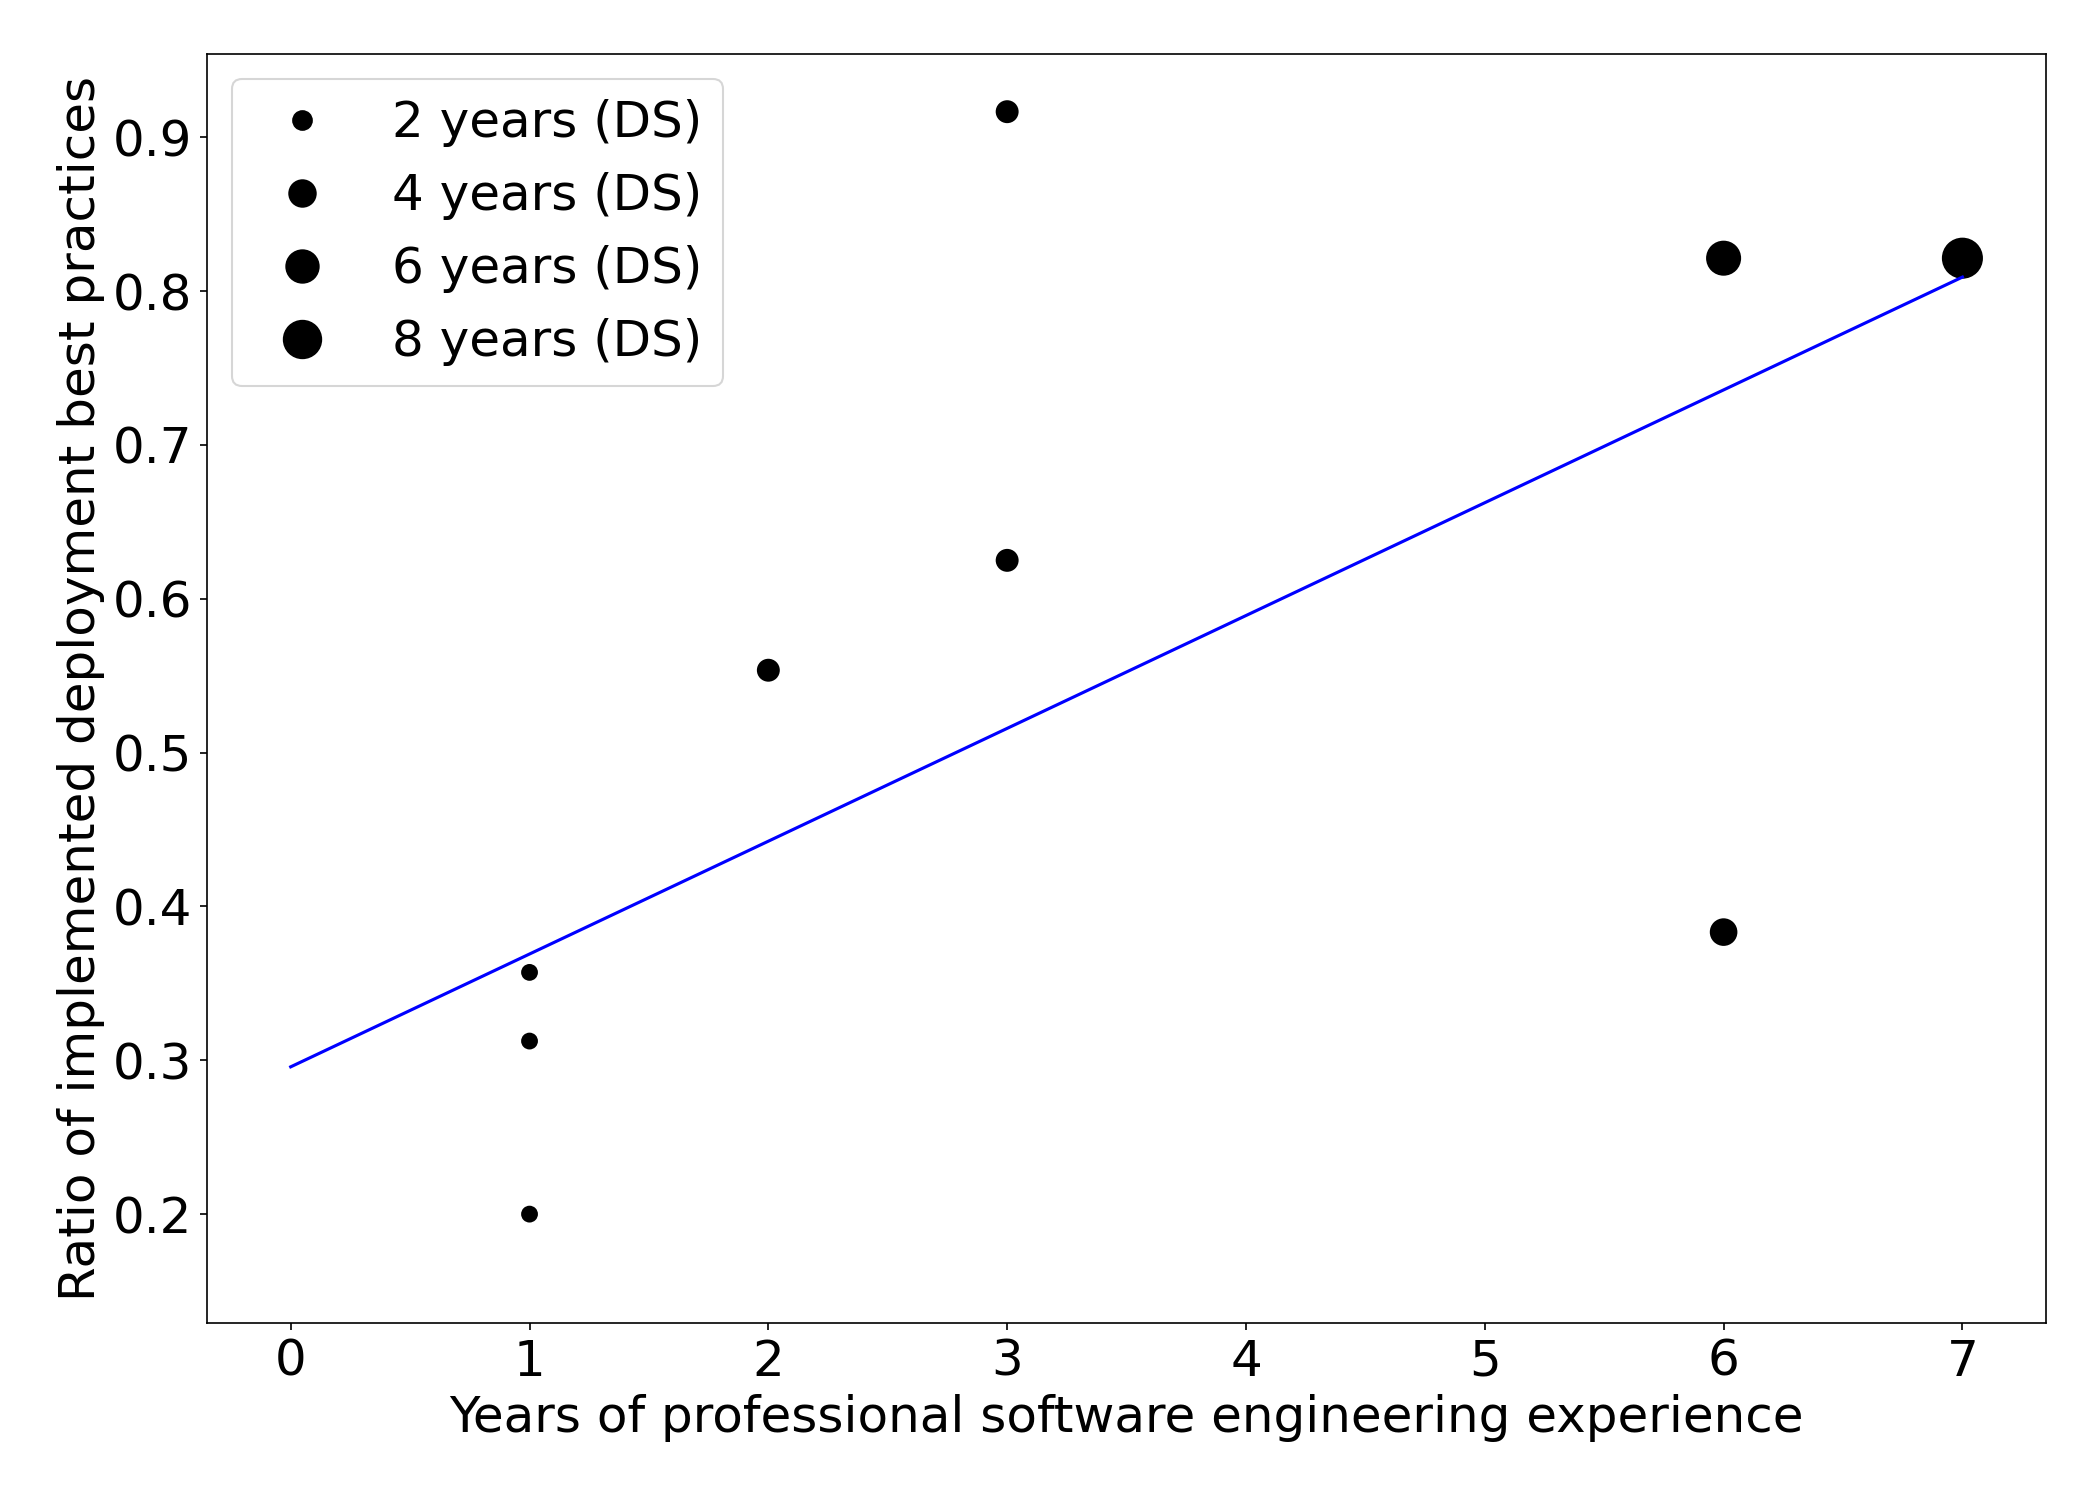
\includegraphics[width=0.7\linewidth]{figures/best-practices.png}
    \captionsetup{width=.9\linewidth}
    \caption{Best practices adoption rate as a function of software engineering experience. The point sizes denote the practitioners' experience in Data Science (DS). The correlation between the axes is $r_{Pearson} = 0.67$ with $p = 0.0033$.}
    \label{fig:adoption}
\end{figure}

\subsection{Technology acceptance}

Participants filled out a form (shown in Appendix \ref{appendix:questions}) after finishing their first deployment with \textit{GreatAI} to provide data for creating the technology acceptance model of the problem context. The survey contained 12 questions from 3 categories, which could be rated on a 7-point Likert scale. Following the methodology of \cite{cruz2019catalog}, the connections between the Perceived Utility (PU), Perceived Ease Of Use (PEOU), and the Intention to use (ITU) were analysed. Only two statistically significant ($P < 0.05$) correlations were uncovered: between PU and ITU ($r_{Pearson} = 0.81$ with $p = 0.0048$); and PEOU and ITU ($r_{Pearson} = 0.80$ with $p = 0.0068$). Learning from the findings of prior case studies, it is reasonable that both the perceived utility and the perceived ease of use play an equally important role in influencing potential clients' intention to use the deployment framework. 

\begin{table}[H]
\centering
\captionsetup{width=.9\linewidth}
\caption{Aggregated results of the TAM survey (sample size = 10) presented in Appendix \ref{appendix:questions}. The values are from a range between 1 and 7.}
\label{table:tam}
{\renewcommand{\arraystretch}{1.2} % for the vertical padding
\begin{tabular}{|c|r|r|r|} \hline
                    & \textbf{Perceived ease of use} & \textbf{Perceived utility} & \textbf{Intention to use} \\\hline
\textbf{Median}     & 5.750                          & 6.375                      & 6.250                     \\\hline
\textbf{Mean}       & 5.450                          & 6.125                      & 5.950                     \\\hline
\textbf{Variance}   & 1.080                          & 0.740                      & 1.747                     \\\hline
\end{tabular}}
\end{table}

The summary of the answers is presented in Table \ref{table:tam}. The value for ease of use lags behind the rest, but it is still quite high. It may be possible that PEOU would go up with further use. Nevertheless, the high perceived utility implies that \textit{GreatAI} shows its value early on. This validates the hypothesis that focusing on good API design is just as important as providing practical features.

\subsection{Task solving \& exit interviews}

To give qualitative depth to the previously presented quantitative results, it is time to discuss the main segment of the interviews. First, the volunteers were requested to skim through the library's documentation beforehand, and they were also given a short verbal overview during the one-on-one meetings. This was followed by having them solve a prepared deployment task\footnote{Available at \href{https://github.com/schmelczer/great-ai-interview-task}{github.com/schmelczer/great-ai-interview-task}.} concerning a similar lifecycle to that presented in the \textit{GreatAI} tutorials. The training part of the task had already been done, the participants only had to deploy a trained classification model.

The participants' backgrounds cover a vast (and incredibly interesting) cross-section of industrial AI/ML use: one of them researched market prediction models for the Hungarian State Treasury, but building an upcoming digital bank's core services, investigating companies' AI use as part of due diligence processes, intrusion detection from network packet traces, creating pose-recognition for people with disabilities, and predicting Sun activity at the European Space Agency are just some of the core activities they have been doing recently. Stemming from this diversity, these semi-structured interviews should provide valuable insights into the generalisability of \textit{GreatAI}.

% The approach used to collect information from interviews and to report data
% is based on the guidelines proposed by Halcomb et al. \cite{halcomb2006verbatim} It is a reflexive,
% iterative process:
% 1. Audio taping of the interview and concurrent note-taking.
% 2. Reflective journaling immediately post-interview.
% 3. Listening to the audiotape and revising memos.
% 4. Triangulation.
% 5. Data analysis.

% The first two authors conducted the interviews, which took approximately one
% hour. We took notes during the interviews and we recorded the interviews with
% the permission of the participants. An example of the notes taken with P09 is
% shown in Fig. 4. This section outlines the main steps of our interview design.
% The full details can be found in our corresponding case study protocol [14].

% Also, the process of memoing assisted
% the researchers to capture their thoughts and interpretations of the interview
% data [44]. The audio recordings could still be used to facilitate a review of
% the interviewers’ performance, and assist interviewers to fill in blank spaces in
% their field notes and check the relationship between the notes and the actual
% responses [12].

% . Thematic analysis is a qualitative data analysis
% method divided into four steps: 1) familiarization with data, 2) generating
% initial labels, 3) reviewing themes, 4) defining and naming themes. This tech-
% nique has been successfully used in previous software engineering studies to
% extract patterns from software [9].

% This step was followed by reviewing themes – step 3 of thematic analysis –
% in which we discussed each label and looked for other labels that could be
% redundant. For example, we merged the labels Feasibility Study and Proof of
% Concept together into a single theme. This step yielded 11 overarching themes
% that we further detail in Section 4.
% -----------------------------

### functionality (PU)
+ You get a lot of features
+ Debugging traces is nice, had some privacy concerns but was easy to find the solution in the docs -> disable\_logging=True
+ it forces you to do Human in the loop
+ Private cloud is very important in banking/treasury
+ Scales well because doesn't depend on 1 DB
+ Utilities good, hate writing feature extraction,  Parallel feature extraction is fascinating, + Great for NLP, should work for other domains if utilities are implemented
+ being extendable very important because if you start using it you get locked into it
+ important to have support for all libs e.g. external matlab
+ Largefile good, haven't heard of other solutions, versioning important -> awareness

### API (PEOU)
- Do data scientists know what decorators are?
- Parameter decorators on the function are bit weird but doesn't know how to do it better
You cannot make an API simpler than the domain but you made it as simple as it could get - Magic save, where does it go? Transparency, balance between too automatic and simple
+ Hates complicated CLI-s, great-ai is very simple
+ Likes Docker, researchers know that
- Won't use if it doesn't work out-of-the-box (this time, it worked, but focusin on the starter code is important)
- Want clickable UI for setting the config - scientists (matlab deployment)

### Whose responsibility is this? (ITU)
- If I had to implement a REST API for a model, I'd do that instead of searching for a lib
Easier to raise awareness if you have a solution

research CD very poor and even industrial projects are sometimes one-man
Cron job runs Matlab script that copies it to the prod env
They used Colab + GitHub + W&B for the treasury -> Add one-click app, heroku
- Already using AWS, sagemaker is preferred

- Trying to appeal to both DS and SE was confusing at first, why training in tutorial if it's a deployment lib
- Whose responsibility is using the lib? - What happens when you have to configure it? 
+ You need so many different experts for a single project, too many, SE is often missing
- AI is mostly used in academy, they have no reason to do good deployment or deployment at all
DS, domain experts don't care about best-practices, End results should look nice, no one cares about behind the scenes
You have to give a value proposition: low maintenance, low cost, better quality
At one company, they had 0 DS people for 3 years, High-level solution can substitute missing professionals imo
Shouldn't care about DS but instead decision-makers because they chose not to hire SE
    + You can have fewer SE-s instead of 0 but still more than 0 and they're effective with great-ai

\subsection{Threats to validity}

\section{Future work} 

The primary purpose of \textit{GreatAI} was to serve as a proxy through which its design decisions could be tested and evaluated in their practical context. For this reason, its design aimed to be a proof-of-principle for validating hypotheses and answering research questions. After successfully doing that, it has been turned into a practical software library suitable for production-use\footnote{\href{https://pypi.org/project/great-ai/}{pypi.org/project/great-ai}}. Although it has already proved its utility, it has also shown that extending its functionality would be worthwhile. Therefore, a number of potential improvements to \textit{GreatAI} are presented below.
 
\subsection{More data science}

The cases presented in Chapter \ref{chapter:case} revolved around NLP. This, unsurprisingly, heavily influenced the design process. The two most notable effects can be found in the REST API's \texttt{/predict} endpoint and some \texttt{utilities} functions. The former is streamlined to accept JSON-compatible data while the latter gives robust feature extraction support for only textual inputs. Supporting the easy, direct upload of larger non-JSON files --- e.g. by saving them to S3 and showing a preview for them on the Dashboard's trace table --- and extending \texttt{utilities} to handle multimedia formats should be sufficient for widely extending the scope of applicability of \textit{GreatAI}.

\subsection{More software engineering}

In order to greatly simplify its API, each \textit{GreatAI} Trace is a single document with a well-defined, multi-level schema that clients can also extend by calling \texttt{log\_metric}. MongoDB provides a convenient (and popular) method for persisting such documents, however, if there is some existing database in the environment, storing Traces in that can be favourable. \href{https://www.postgresql.org/}{PostgreSQL} is a popular choice and it also features good JSON document support. Hence, introducing first-class integration for PostgreSQL could benefit some clients.

As described in Designing Data-intensive Applications \cite{kleppmann2017designing}, services can fall into three broad categories: online systems, batch processing, and stream processing (near-teal-time systems). As of yet, \textit{GreatAI} only provides streamlined support for the first two. Thus, developer experience could be improved by providing simple, direct integration with popular message queues/protocols, such as \href{https://kafka.apache.org/}{Apache Kafka} \cite{kreps2011kafka}, \href{https://aws.amazon.com/sqs/}{AWS SQS} \cite{garfinkel2007evaluation}, or \href{https://www.amqp.org/}{AMQP} \cite{vinoski2006advanced}.

Some metrics of \textit{GreatAI}, such as the cache statistics, versions, and derived data from traces can be already conveniently queried from its REST API. Nevertheless, adding support for the de facto standard metric gathering tool \href{https://prometheus.io/}{Prometheus} could save the library's users from one more integration step.

The common theme among the above-mentioned opportunities is that they could be reasonably well implemented without any user input, making them in line with the library's philosophy. Of course, the open-source nature of \textit{GreatAI} also allows anyone to already provide support for a wide range of integrations. Additionally, the scope could be also reasonably extended, i.e. more practices could be covered by including more criteria next to the GREAT ones.
